% generated by scripts/aggregate_budget.py -- do not edit by hand
% needs \usepackage{pgfplots} and \pgfplotsset{compat=1.18} in the preamble
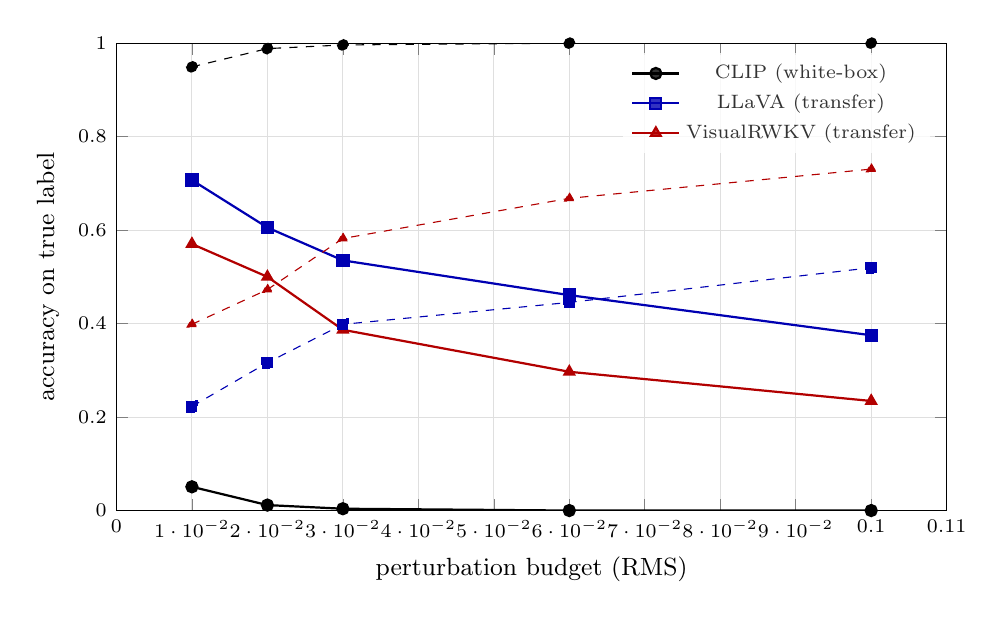
\begin{tikzpicture}
\begin{axis}[
  width=\columnwidth, height=0.62\columnwidth,
  xlabel={perturbation budget (RMS)}, ylabel={accuracy on true label},
  xmin=0, ymin=0, ymax=1,
  legend style={font=\scriptsize, at={(0.98,0.98)}, anchor=north east, draw=none, fill opacity=0.8},
  tick label style={font=\scriptsize}, label style={font=\small},
  grid=major, grid style={gray!25},
]
\addplot[black,      mark=*, thick] coordinates {(0.010,0.0508) (0.020,0.0117) (0.030,0.0039) (0.060,0.0000) (0.100,0.0000)};
\addlegendentry{CLIP (white-box)}
\addplot[blue!70!black, mark=square*, thick] coordinates {(0.010,0.7070) (0.020,0.6055) (0.030,0.5352) (0.060,0.4609) (0.100,0.3750)};
\addlegendentry{LLaVA (transfer)}
\addplot[red!70!black,  mark=triangle*, thick] coordinates {(0.010,0.5703) (0.020,0.5000) (0.030,0.3867) (0.060,0.2969) (0.100,0.2344)};
\addlegendentry{VisualRWKV (transfer)}
\addplot[black,      mark=*, dashed, thin, forget plot] coordinates {(0.010,0.9492) (0.020,0.9883) (0.030,0.9961) (0.060,1.0000) (0.100,1.0000)};
\addplot[blue!70!black, mark=square*, dashed, thin, forget plot] coordinates {(0.010,0.2227) (0.020,0.3164) (0.030,0.3984) (0.060,0.4453) (0.100,0.5195)};
\addplot[red!70!black,  mark=triangle*, dashed, thin, forget plot] coordinates {(0.010,0.3984) (0.020,0.4727) (0.030,0.5820) (0.060,0.6680) (0.100,0.7305)};
\end{axis}
\end{tikzpicture}
